 %\documentstyle [10pt,amsmath,amsfonts]{article}
\documentclass [10pt] {article}
\addtolength{\oddsidemargin}{-.75in}
\addtolength{\evensidemargin}{-.75in}
\addtolength{\textwidth}{1.5in}
\addtolength{\topmargin}{-.75in}
\addtolength{\textheight}{1.5in}

\usepackage{amsfonts}      
\usepackage{amsmath}
\usepackage{amssymb} 
\usepackage{amsthm}
\usepackage{bm}
\usepackage{graphicx}
\usepackage{enumerate}
\usepackage{mathrsfs}
%\usepackage{tikz}
\usepackage{multicol}
\usepackage[dvipsnames]{xcolor}
\usepackage{gensymb}
\usepackage{ulem}
\makeatletter
\renewcommand*\env@matrix[1][c]{\hskip -\arraycolsep
  \let\@ifnextchar\new@ifnextchar
  \array{*\c@MaxMatrixCols #1}}
\makeatother
\usepackage{hyperref}
\hypersetup{
    colorlinks=true,
    linkcolor=blue,
    filecolor=magenta,      
    urlcolor=cyan,
    pdftitle={Overleaf Example},
    pdfpagemode=FullScreen,
    }
\usepackage{minted}
\usemintedstyle{borland}
\usepackage{xcolor} % to access the named colour LightGray
\definecolor{LightGray}{gray}{0.9}

\newcommand{\R}{\mathbb{R}}
\newcommand{\Z}{\mathbb{Z}}
\newcommand{\Q}{\mathbb{Q}}
\newcommand{\N}{\mathbb{N}}
\newcommand{\C}{\mathbb{C}}
\newcommand{\M}{\mathbb{M}}
\newcommand{\ltset}{\mathcal{L}}
\newcommand{\ov}{\overline}
\newcommand{\con}{\overline}
\newcommand{\union}{\bigcup}
\newcommand{\intersect}{\bigcap}
\newcommand{\trace}{\mathrm{tr}}
\newcommand{\dash}{\textemdash}
\newcommand{\eps}{\epsilon}
\newcommand{\Stab}{\mathrm{Stab}}
\newcommand{\im}{\mathrm{Im}}
\newcommand{\Hom}{\mathrm{Hom}}
\newcommand{\Aut}{\mathrm{Aut}}
\newcommand{\Inn}{\mathrm{Inn}}
\newcommand{\End}{\mathrm{End}}
\newcommand{\norm}{\triangleleft}
\newcommand{\normeq}{\trianglelefteq}
\newcommand{\ds}{\displaystyle}
\newcommand{\Var}{\mathrm{Var}}
\newcommand{\Cov}{\mathrm{Cov}}
\newcommand{\bin}{\mathrm{bin}}
\newcommand{\supp}{\mathrm{supp}}
\newcommand{\sgn}{\mathrm{sgn}}
\newcommand{\unif}{\mathrm{unif}}
\newcommand{\Bern}{\mathrm{Bern}}
\newcommand{\ul}{\underline}
\newcommand{\lcm}{\mathrm{lcm}}
\newcommand{\Perm}{\mathrm{Perm}}
\newcommand{\Core}{\mathrm{Core}}
\newcommand{\ess}{\text{ess}}
\newcommand{\E}{\mathbb{E}}
\newcommand{\median}{\mathrm{median}}
\renewcommand{\P}{\mathbb{P}}
\renewcommand{\phi}{\varphi}

\renewcommand{\emptyset}{\varnothing}

\begin{document}
{\noindent}ECS 256 - Professor N. Matloff\hfill Group: Yun Qin, Jane Park\\
Fall 2022\hfill 20 October 2022
\begin{center}{\Large Problem Set 1}\end{center}
\begin{enumerate}
\item[{\bf1.}] {\it Consider a finite-state space, aperiodic Markov chain with transition matrix $P$. Our textbook shows a way to find the stationary probability vector $\pi$ that is alternative to the usual method that solves a system of linear equations. Say the matrix is of size $r\times r$. The thrust of the argument is as follows:}
\begin{enumerate}
\item[$\bullet$]{\it The power $P^k$ is the $k$-step transition matrix.}
\item[$\bullet$]{\it So, row 1 of the matrix is $\P[X_k = j | X_0 = 1]$, $j = 1,\cdots,r$. Row 2 is $\P[X_k = j | X_0 = 2]$, $j = 1,\cdots,r$, and so on.}
\item[$\bullet$]{\it We know that for an aperiodic chain, $\ds\lim_{k\to\infty}\P[X_k = j | X_0 = i]\to\pi_j$.}
\item[$\bullet$]{\it Thus for large $k$, each row of $P^k$ will be approximately the vector $\pi'$.}
\item[$\bullet$]{\it So, to find $\pi$, we could raise $P$ to a large power, then use row 1 as $\pi$.}
\item[$\bullet$]{\it But even better, we could average all the rows, which presumably will give us a better estimate.}
\end{enumerate}
{\it Investigate the accuracy of this approach, as follows:}
\begin{enumerate}
\item[$\bullet$]{\it Do your experiments for one small $P$ and one large one, of your choice.}
\item[$\bullet$]{\it For values of $k = 1,2,3,\cdots,m$ (your choice of $m$): Find the estimates of $\pi$, both using row 1 only and averaging all the rows. Take as your accuracy criterion the $\ell^1$ distance (sum of absolute differences) of the estimated $\pi$ to the actual value.}
\item[$\bullet$]{\it Show your results graphically, with commentary in a }\texttt{.tex} {\it file.}
\end{enumerate}

\begin{figure}[h]
    \centering
    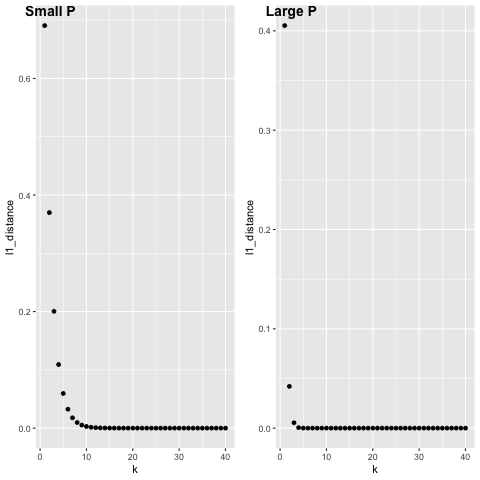
\includegraphics[width=0.6\textwidth]{problem1.png}
    \caption{Convergent trend of the $\ell^1$-norm difference over powers $k=1,\cdots,m$ of $(P^k)[1,]$ and our $\pi_k$ (defined below). We set \texttt{m=40}. (Left to right) \texttt{ggplots} of the desired compared quantities for $3\times3$ transition matrix example; and of our $20\times20$ transition matrix example, respectively.}
\end{figure}

Notice that the graphs, for both small and large dimensional $P$, we have a quick deflation of the difference between the first row of $P^k$, and $\pi_k$ where $\ds\pi_k[j]:=\frac{1}{r}\sum_{j=1}^rP^k[,j]$, $\ds\lim_{k\to\infty}\|P^k[1,]-\pi_k\|_{\ell^1}=\lim_{k\to\infty}\sum_{j=1}^r\left|P^k[1,j]-\pi_k[j]\right|$. This implies that we have convergence of $P^k[1,]$ to $\pi_k$, as $k\to\infty$. I.e.:
$$\lim_{k\to\infty}P^k[1,]=\lim_{k\to\infty}\pi_k=:\pi.$$
Conceptually, we know that the transition matrix always has 1 as an eigenvalue, and that te corresponding left eigenvector is the stationary distribution in vector form, given by $\pi$. The transition matrix has its full set of eigenvectors comprise of its eigenbasis, and all eigenvalues aside from 1 are values in $[0,1)\subset\R$. This implies that as we take higher powers of $P$, all eigenvalues not 1 vanish. This means that we have a Rank 1 matrix, entailing that all rows are multiples of each other. Thus, taking the average of all column entry for higher $k$ powers will only make entries of $\pi_k$ converge to the desired stationary probability distribution, put in vector form.

One thing we noticed is that for the larger $P$, which rows of twenty entries are taken from a $\mathrm{Unif}[1,20]$ distribution, and which sum we normalized (so that the sum of any row is 1 to fulfill that requirement for the definition of transition matrices), the more spread out the values are in that matrix, and the (possibly significantly) smaller each row entry will be in subsequent powers of that matrix. This is why, in our case, we have many data points far above the $y=0$ line in our $3\times3$ case whereas in the $20\times20$ case, we only had three points for $k=1,2,3$ where the distance between $P^k[1,]$ and $\pi_k$ is noticeably greater than 0.
\item[{\bf2.}] {\it Consider the states of a Markov chain over time, $X_0, X_1, X_2, \cdots$, with the state space being some subset of the set of all integers, which we will take to be $1,\cdots,m$. Suppose the chain has a stationary distribution $\pi$, and that $X_0$ has this distribution.

There is a term from time series analysis, autocorrelation: $\rho(k)$, defined to be the correlation between $X_i$ and $X_{i+k}$. Note that this quantity depends only on $k$, not $i$.}
\begin{enumerate}
\item[{\bf(a)}] {\it Explain why there is no dependence on $i$ (}\texttt{.tex} {\it file).}
Let $P\in[0,1]^{m\times m}$ denote the transition matrix from any state $i$ to state $j$ for $i,j\in\{1,\cdots,m\}$.

If $\pi$ is the stationary distribution, then as a vector $[\pi]\in[0,1]\in\R^m$, we have that $[\pi]'\cdot P = [\pi]' = 1\cdot[\pi]'$ (meaning that $\pi$ is a left eigenvector to $P$). Since $X_0\sim\pi$, so that $\P[X_0=j]:=\pi(j)$. We have that, since for all $n$, $X_n$ has the same distribution as is suggested by the vector $[\pi]'\cdot P^{n}=1^n\cdot[\pi]'=[\pi]$, so that $X_n\sim\pi$ for all $n\in\Z_{\ge0}$. This implies that $\ds\mu_{X_n}=\mu_{X_0}=:\mu$, and $\ds\sigma_{X_n}=\sigma_{X_0}=:\sigma$ for all $n\in\Z_{\ge0}$.

Since these distributions $X_n$ form a Markov chain, we know that the probability of $X_{i+k}$ achieving state $t$ given that $X_i$ is at state $i$, for $i,i+k\in\{1,\cdots,m\}$ is
\begin{equation}\P[X_{i+k}=t|X_i=s]=\P[X_k=t|X_0=s]=(P^k)_{st}.\end{equation}

Then the autocorrelation of $X_i$ and $X_{i+k}$ is:
\begin{align*}
\rho(X_i,X_{i+k})&:=\frac{\E[X_iX_{i+k}]-\mu_{X_i}\mu_{X_{i+k}}}{\sigma_{X_i}\sigma_{X_{i+k}}}\\
&=:\frac{\E[X_iX_{i+k}]-\mu^2}{\sigma^2},&&\text{as all $X_n$ are identically distributed;}\\
&=\frac{\ds\sum_{s=1}^m\P[X_i=s]\E[X_iX_{i+k}|X_i=s]-\mu^2}{\sigma^2},&&\text{by the {\bf Law of Total Expectation};}\\
&=\frac{\ds\sum_{s=1}^m\pi[s]\E[sX_{i+k}|X_i=s]-\mu^2}{\sigma^2},&&\text{as }\P[X_i=s]=\P[X_0=s]=\pi[s];\\
&=\frac{\ds\sum_{s=1}^m s \ \pi[s]\E[X_{i+k}|X_i=s]-\mu^2}{\sigma^2},&&\text{by linearity of expectation;}\\
&=\frac{\ds\sum_{s=1}^m s\pi[s]\sum_{t=1}^m t\P[X_{i+k}=t|X_i=s]-\mu^2}{\sigma^2}\\
&=\frac{\ds\sum_{t=1}^m\sum_{s=1}^m st \ \pi[s]\P[X_{i+k}=t|X_i=s]-\mu^2}{\sigma^2},&&\text{as finite sums are reorderable;}\\
&=\frac{\ds\sum_{t=1}^m\sum_{s=1}^m st \ \pi[s](P^k)_{st}-\mu^2}{\sigma^2},&&\text{by (1) above.}
\end{align*}
Focusing on the first summand in the numerator, we observe that this expression linearly standardizes $\E[X_iX_{i+k}]=\E[X_0X_k]$, for all $k\in\Z^+$.

The expression $\ds\E[X_0X_k]=\sum_{t=1}^m\sum_{s=1}^m s \pi[s] \cdot t \ (P^k)_{st}$, which is akin to the {\it Hadamaard product} of $\ds[s]_{s=1}^m$ and $\ds[\pi]$, denoted $\ds[s]_{s=1}^m\circ[\pi]:=[s\cdot\pi[s]]_{s=1}^m$, dotted with $[t(P^k)_{st}]_{s=1}^m$, which is $t$-times the $t^\text{th}$ column of $P^k$, summed over $t=1,\cdots,m$, which is a multivariate expectation of the product random variable $X_0X_k$, where $X_k$ depends on $X_0$.
\item[{\bf(b)}]{\it Write an} \texttt{R} {\it function with call form}
\texttt{MCautocor(k,P)}
{\it(Note that an argument} \texttt{m} {\it is not needed. Explain why.)}

The argument $m$ is unnecessary because the conception of $m$ is built into the dimension of the matrices side (equal by design of the transition matrix). In other words, the transition matrix already tells us the number of states for our random variable{\dash}which $m$ denotes.
\end{enumerate}
\item[{\bf3.}]{\it Consider the ALOHA model with 3 stations. Derive the long- run average time between collisions. Expression your answer in terms of $p$, $q$ and $\pi$, and evaluate for the case $p = 0.4$, $q = 0.3$. Show your reasoning in a} \texttt{.tex} {\it file.}

The long-run average time of collisions would be, for any given trial in this scenario, the quantity time units divided by the number of collisions that occur in that trial.

The long running average of the number of collisions is determined by $\ds\P[C]$ per epoch [time unit], where $\ds\P[C]$ is the $\P$robability of $C$ollisions. By {\bf the law of total probability}, $\ds\P[C]=\sum_{i=0}^3\P[C|S=i]\P[S=i]$, where $S$ is denotes the current state of the system. If you are given that you are at State $i$, we need only care about the summands in each $P_{ij}$ which contains a $p^2$ or $p^3$ in the product, where $P_{ij}$ is the entry in the $(i,j)$ position of $P$, for each fixed $i$ and $j=0,1,2,3$. This is because those terms with $p^2$ or $p^3$ denote times when there are 2 or 3 active nodes attempting to send a message at the same time, respectively. If more than one node attempts to send a message, we then have a collision.

Thus:
\begin{align*}
\P[C|S=0]&=\binom{3}{2}q^2(1-q)p^2+q^3p^3+\binom{3}{2}q^{3}(1-p)p^2\\
\P[C|S=1]&=\binom{2}{1}q(1-q)p^2+q^2p^3+\binom{3}{2}q^2p^2(1-p)\\
\P[C|S=2]&=(1-q)p^2+qp^3+\binom{3}{2}q(1-p)p^2\\
\P[C|S=3]&=p^3+\binom{3}{2}p^2(1-p).
\end{align*}

And $\P[S=i]=\pi[i]$, where $\pi$ is the eigenvector of eigenvalue 1 for $I_4-P'$, which are the stationary state probabilities of the ALOHA model.

So for $p=0.4$ and $q=0.3$ this sum  $\ds\P[C]=\sum_{i=0}^3\P[C|S=i]\P[S=i]=0.1791231$, according to our \texttt{Problem3.R}.

By the Markov property in Equation (1) in {\bf1.} above, we have that we have, on average, $\P[C]$ collisions happen with ever next epoch. Thus, if we run over some sufficiently large $N$ epochs [time unit], we will have around $N\P[c]$ collisions. The the average time between collisions over these $N$ epochs is $$\lim_{N\to\infty}\frac{N}{N\P[C]}=\lim_{N\to\infty}\frac{1}{\P[C]}=\frac{1}{0.1791231}=5.582754.$$
Thus, we have on average $5.58$ epochs between each collision for our ALOHA net with 3 stations.
\item[{\bf4.}]{\it Consider a Markov chain with finite state space.}
\begin{enumerate}
\item[{\bf(a)}]{\it Write an} \texttt{R} {\it function with call form}\\
\texttt{eTij(P)  \# P is the transition matrix}\\
{\it giving the values of $ET_{ij}$.}

This is given in our \texttt{Problem4.R}.
\item[{\bf(b)}]{\it Do the same for variance, writing a function}\\
\texttt{varTij(P)  \# P is the transition matrix}\\
{\it that finds all Var(Tij), where Tij is the same it takes to go from state i to state j. Show your derivation in a} \texttt{.tex} {\it file.}

The derivation is as follows: Given $d$ states, fix $i,j\in\{1,\cdots,d\}$.

We already have the expression $\E[T_ij]$, as given by our function \texttt{ETij(P)} in our \texttt{Problem4.R}. That quantity squared will be part of our second summand in the formula, \begin{equation}\Var(T_{ij})=\E[T_{ij}^2]-\E[T_{ij}]^2.\end{equation}
Then the problem lies with $\E[T_{ij}^2]$. This term is derived by definition of $T_{ij}$ given $U=k\in\{1,\cdots,d\}$, the next step after ``starting" at State $i$. We still have that if given $U=j$, then $T_{ij}^2\equiv1^2=1$. Now, if we're given $U=k\ne j$
$$T_{ij}^2=(1+T_{kj})^2 \ \ \ \ \text{for }k\in\{1,\cdots,d\}\setminus\{j\}.$$
Thus, for all $i,j\in\{1,\cdots,d\}$:
\begin{align*}
    \E[T_{ij}^2]&=\sum_{k=1}^d p_{ik}\E[T_{ij}^2|U=k],&&\text{by {\bf Total Law of Expectation};}\\
    &=p_{jj}\E[T_{jj}^2]+\sum_{k\ne j}p_{ik}\E[(1+T_{kj})^2],&&\text{using {\bf PSB Equation (6.39)};}\\
    &=p_{jj}+\sum_{k\ne j}p_{ik}\E[1+2T_{kj}+T_{kj}^2],&&\text{by above paragraph, $\E[T_{jj}^2]\equiv1$;}\\
    &=p_{jj}+\sum_{k\ne j}p_{ik}\left(1+2\E[T_{kj}]+\E[T_{kj}^2]\right),&&\text{by linearity of expectation;}\\
    &=p_{jj}+\sum_{k\ne j}p_{ik}+2\sum_{k\ne j}p_{ik}\E[T_{kj}]+\sum_{k\ne j}\E[T_{kj}^2]\\
    &=1+2\sum_{k\ne j}p_{ik}\E[T_{kj}]+\sum_{k\ne j}\E[T_{kj}^2]\\
    &=2\left(1+\sum_{k\ne j}p_{ik}\E[T_{kj}]\right)-1+\sum_{k\ne j}\E[T_{kj}^2],&&\text{the ol' ``add zero" trick;}\\
    &=2\E[T_{ij}]-1+\sum_{k\ne j}\E[T_{kj}^2],&&\text{by {\bf PSB Equation (6.41)}.}
\end{align*}
Here let $\beta_i$ denote $E(T_{in}^2)$, and define $\beta=(\beta_1, \beta_2,...,\beta_{n-1})'$, so we have
\begin{equation}
    \beta_i = 2E[T_{in}]-1+\beta_k
\end{equation}
Equation (3) is a system of linear equations, which we can write in matrix form. Then the code to solve the system is in our \texttt{Problem4.R} function \texttt{findbeta}.

Then, using Equation (2) above, we conclude that:
$$\Var(T_{ij})=\sum_{k\ne j}\E[T_{kj}^2] \ \ -\E[T_{ij}]^2+2\E[T_{ij}]-1.$$
The function \texttt{varTij(P)} in our \texttt{Problem4.R} uses this forulation to return the value of $\Var(T_{ij})$, for any transition matrix \texttt{P}.
\end{enumerate}
\end{enumerate}
\end{document}

MCAutocor <- function(k,P) #k an integer; P a transition matrix
{
  EX0Xk <- 0
  pi <- findpi(P)
  #pi <- solve(I-P,rep(0,m))
  #if(sum(pi) <= 0){
  #  pi <- -1*pi
  #}
  m <-nrow(P)
  mu <- sum((1:m)*pi)
  sigma2 <- sum((1:m)^2*pi)-mu^2
  Pk <- P
  if (k > 1){
    for(j in 1:(k-1)){
      Pk <- Pk %*% P
    }
  }
  for (t in 1:m) {
    for (s in 1:m) {
      EX0Xk <- EX0Xk + s*t*pi[s]*Pk[s,t]
    }
  }
  (EX0Xk-mu^2)/(sigma2)
}
